\vspace{-1.5em}
\section{Related Work}
\label{sec:related}
\vspace{-1em}

\subsubsection{2D Video Object Segmentation.}
Video object segmentation (VOS) segments and tracks target objects across video sequences with temporally coherent masks~\cite{perazzi2016benchmark, caelles2017one, voigtlaender2019feelvos, maninis2018video, wu2025denver}. Early approaches relied on appearance propagation or optical flow but struggled with long-term consistency and occlusion~\cite{yang2019video, oh2019video, bhat2020learning}. Recent memory-based architectures leverage spatio-temporal attention and feature retrieval for improved object association~\cite{yang2021associating, cheng2022xmem, cheng2021rethinking, liu2022learning, park2022per, xu2022reliable, yang2024scalable, yang2022decoupling, li2024univs, cheng2024putting}, with subsequent work improving memory efficiency via restricted banks~\cite{zhou2024rmem}, gated linear matching~\cite{liu2025livos}, unified transformer frameworks~\cite{li2024onevos, zhang2025jointformer}, and dynamic anchor queries~\cite{zhou2024improving}. New benchmarks~\cite{hong2023lvos} and specialized settings such as panoramic video~\cite{yan2024panovos} and point-based prompting~\cite{mahadevan2024point} further broaden the evaluation landscape.

SAM2~\cite{ravi2024sam2}, a promptable model with streaming memory, achieves strong results across benchmarks. Follow-up efforts extend SAM2 with memory trees for long-range identity preservation~\cite{ding2024sam2long}, distractor-aware updates~\cite{videnovic2025distractor}, on-device efficiency~\cite{zhou2025edgetam}, text-driven understanding~\cite{cuttano2025samwise}, and other improvements~\cite{yang2024samurai, yang2025mosam, ye2025entitysam}. Concurrent work further combines SAM2 with large language models for reasoning-based segmentation~\cite{yuan2025sa2va, yan2024visa, bai2024one}. Despite these advances, large viewpoint changes, occlusion, and disappearance-reappearance events cause significant degradation~\cite{ding2025mosev2, xu2018youtube, perazzi2017davis}. Our method addresses these limitations by integrating 3D-aware representations into SAM2 for object-consistent segmentation under challenging viewpoint and appearance variations.

\vspace{-1em}
\subsubsection{3D Instance Segmentation.}
Mainstream 3D instance segmentation follows two tracks. Proposal-centric methods predict instance masks from point clouds with learned proposals~\cite{schult2022mask3d, jiang2020pointgroup, han2020occuseg, vu2022softgroup, misra2021end, sun2023superpoint, kolodiazhnyi2024oneformer3d, takmaz2023openmask3d, piekenbrinck2025opensplat3d}, with recent extensions adding promptable segmentation~\cite{zhou2024point} and fast open-vocabulary recognition~\cite{boudjoghra2025openyolo}. A complementary line lifts 2D results to 3D by projecting per-view masks and merging across views~\cite{yang2023sam3d, xu2024embodiedsam, nguyen2024open3dis, boudjoghra2024open, jung2025details, xu2023neurallift, kerr2023lerf, vora2021nesf, jiang2024open, bautista2022gaudi, hsu2025openm3d, tu2023imgeonet, li2024genrc}, employing superpoint affinity~\cite{yin2024sai3d}, zero-shot feature distillation~\cite{wang2024lift3d, engelmann2024opennerf}, hierarchical contrastive learning~\cite{ying2024omniseg3d, kim2024garfield}, and egocentric Gaussian lifting~\cite{gu2024egolifter}, but still depending on posed RGB-D for mask consolidation.

The rise of 3D Gaussian Splatting has further enabled semantic scene representations by distilling foundation-model features into Gaussians~\cite{qin2024langsplat, zhou2024feature, wu2024opengaussian, peng20243d}, assigning per-Gaussian identity encodings~\cite{ye2024gaussian, zhai2025panogs}, solving 2D-to-3D label assignment optimally~\cite{shen2024flashsplat}, and unifying lifting with segmentation end-to-end~\cite{zhu2025rethinking}. However, pure 2D promptable segmentation rarely suffices for 3D instances because cross-view consistency is not enforced, leading to view-inconsistent masks and fragmented instances~\cite{zhao2025sam2object, xu2024embodiedsam, peng2023openscene, takmaz2023openmask3d, jia2024sceneverse}. Our approach instead imposes 3D-aware self-consistency directly on video, preserving identity and geometry without 3D annotations or point-cloud mask merging.


\begin{figure*}[t]
  \centering
\vspace{-3mm}
  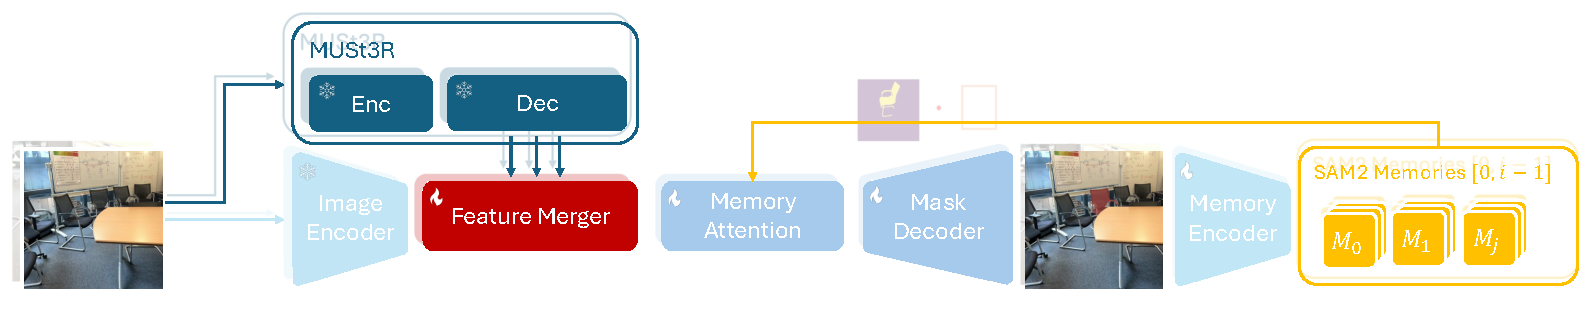
\includegraphics[width=\linewidth]{figs/pipeline.pdf}
  \vspace{-6mm}
  \caption{\textbf{3AM Pipeline Overview.} 
  Our Feature Merger fuses multi-level MUSt3R features, learned from multi-view consistency to encode implicit geometric correspondence, with SAM2's appearance features via cross-attention and convolutional refinement. These merged geometry-aware representations then undergo memory attention with previous frames and mask decoding, enabling spatially-consistent object recognition that maintains identity across large viewpoint changes without requiring camera poses at inference.
  }
  \label{fig:pipline}
\vspace{-3mm}
\end{figure*}


\vspace{-1em}
\subsubsection{End-to-End 3D-Aware Methods.}
Recent end-to-end 3D reconstruction models directly infer geometric structure from 2D inputs~\cite{cabon2025must3r, wang2024dust3r, wang2025continuous, wang2025vggt, yang2025fast3r, chen2025long3r, leroy2024grounding, wu2025point3r, charatan2024pixelsplat, ye2024no, wang20243d, lin2025longsplat, shih2025prior, fan2025spectromotion, liu2023robust, su2024boostmvsnerfs}. The DUSt3R/MASt3R family has been extended to dynamic scenes~\cite{zhang2024monst3r}, incremental reconstruction with spatial memory~\cite{wang20253d}, feed-forward Gaussian splatting~\cite{smart2024splatt3r}, efficient multi-view fusion~\cite{tang2025mv}, real-time dense SLAM~\cite{murai2025mast3r}, unconstrained structure-from-motion~\cite{duisterhof2025mast3r}, and training-free 4D reconstruction~\cite{chen2025easi3r}. Feed-forward models now also jointly predict geometry and semantics~\cite{fan2024large, sun2025uni3r, jiang2025gausstr}, with studies analyzing how different foundation models contribute complementary 3D capabilities~\cite{man2024lexicon3d}.

This progress has fueled end-to-end 3D-aware segmentation frameworks~\cite{jain2024odin, Jayanti2025SegMASt3R, li2025ovseg3r}. PanSt3R~\cite{zust2025panst3r} integrates 3D-aware features from MUSt3R~\cite{cabon2025must3r} with a transformer decoder for joint geometry and panoptic segmentation via learnable quadratic fusion. However, it is incompatible with promptable backbones (\eg, SAM2), limiting interactivity, and requires offline access to entire sequences, preventing streaming. 



% \section{Related Work}
% \label{sec:related}

% \subsubsection{2D Video Object Segmentation.}
% Video object segmentation (VOS) segments and tracks target objects across video sequences with temporally coherent masks~\cite{perazzi2016benchmark, caelles2017one, voigtlaender2019feelvos, maninis2018video, wu2025denver}. Early approaches relied on appearance propagation or optical flow but struggled with long-term consistency and occlusion~\cite{yang2019video, oh2019video, bhat2020learning}. Recent memory-based architectures leverage spatio-temporal attention and feature retrieval for improved object association~\cite{yang2021associating, cheng2022xmem, cheng2021rethinking, liu2022learning, park2022per, xu2022reliable, yang2024scalable, yang2022decoupling, li2024univs, cheng2024putting}. SAM2~\cite{ravi2024sam2}, a promptable model with streaming memory supporting points, boxes, and masks, achieves strong results across benchmarks. Follow-up efforts extend SAM2~\cite{yang2024samurai, yang2025mosam, ye2025entitysam, ding2024sam2long, videnovic2025distractor}: SAM2Long~\cite{ding2024sam2long} introduces memory trees for long-range identity preservation, while DAM4SAM~\cite{videnovic2025distractor} incorporates distractor-aware updates for cluttered scenes. Despite these advances, large viewpoint changes, occlusion, and disappearance-reappearance events cause significant degradation, as shown by MOSEv2~\cite{ding2025mosev2, xu2018youtube, perazzi2017davis}. To address these limitations, our method integrates 3D-aware representations into SAM2 for object-consistent segmentation under challenging viewpoint and appearance variations.

% \subsubsection{3D Instance Segmentation.}
% Mainstream 3D instance segmentation follows two tracks. Proposal-centric methods operate natively in 3D, predicting instance masks from point clouds with learned proposals, often requiring large-scale 3D supervision and suffering from domain shifts~\cite{schult2022mask3d, jiang2020pointgroup, han2020occuseg, vu2022softgroup, misra2021end, sun2023superpoint, kolodiazhnyi2024oneformer3d, takmaz2023openmask3d, piekenbrinck2025opensplat3d}. A complementary line lifts 2D results to 3D by projecting per-view masks and merging across views, but still depends on posed RGB-D and point clouds for mask consolidation~\cite{yang2023sam3d, xu2024embodiedsam, nguyen2024open3dis, boudjoghra2024open, jung2025details, xu2023neurallift, kerr2023lerf, vora2021nesf, jiang2024open, bautista2022gaudi, hsu2025openm3d, tu2023imgeonet, li2024genrc}. Pure 2D promptable segmentation rarely suffices for object-aligned 3D instances because cross-view association and temporal consistency are not enforced by image-space inference alone. Consequently, multi-view fusion often exhibits view-inconsistent masks, error accumulation, and fragmented 3D instances~\cite{zhao2025sam2object, xu2024embodiedsam, peng2023openscene, takmaz2023openmask3d, jia2024sceneverse}. In contrast, our approach imposes 3D-aware self-consistency directly on video, preserving identity and geometry without 3D annotations or point-cloud mask merging.


% \begin{figure*}[t]
%   \centering
%   % \vspace{-3mm}
%   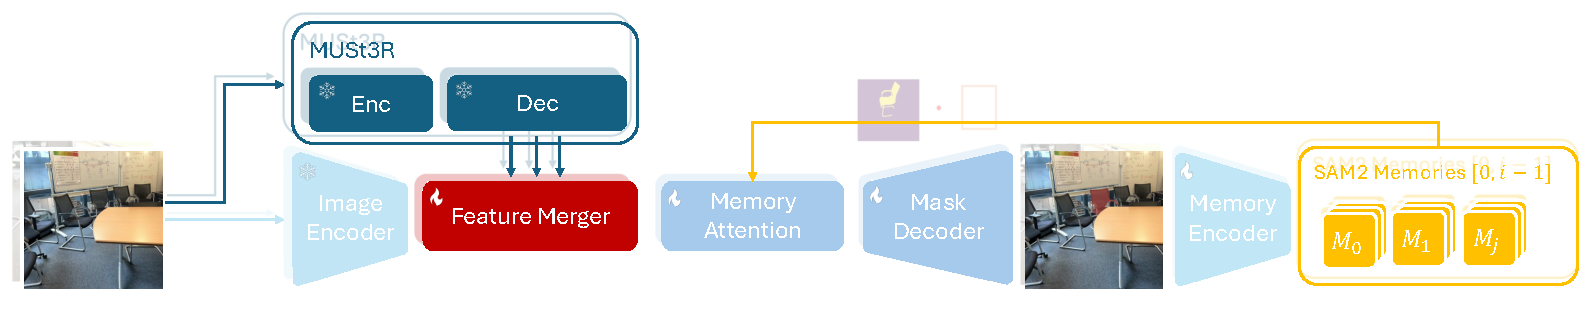
\includegraphics[width=\linewidth]{figs/pipeline.pdf}
%   \vspace{-6mm}
%   \caption{\textbf{3AM Pipeline Overview.} 
%   Our Feature Merger fuses multi-level MUSt3R features, learned from multi-view consistency to encode implicit geometric correspondence, with SAM2's appearance features via cross-attention and convolutional refinement. These merged geometry-aware representations then undergo memory attention with previous frames and mask decoding, enabling spatially-consistent object recognition that maintains identity across large viewpoint changes without requiring camera poses at inference.
%   }
%   \label{fig:pipline}
% \end{figure*}


% \subsubsection{End-to-End 3D-Aware Methods.}
% Recent progress in end-to-end 3D reconstruction shows modern models can directly infer geometric structure from 2D inputs, enhancing downstream 3D perception tasks~\cite{cabon2025must3r, wang2024dust3r, wang2025continuous, wang2025vggt, yang2025fast3r, chen2025long3r, leroy2024grounding, wu2025point3r, charatan2024pixelsplat, ye2024no, wang20243d, lin2025longsplat, shih2025prior, fan2025spectromotion, liu2023robust, su2024boostmvsnerfs}. This has fueled end-to-end 3D-aware segmentation frameworks that unify geometric reasoning and object parsing~\cite{jain2024odin, Jayanti2025SegMASt3R, li2025ovseg3r}. PanSt3R~\cite{zust2025panst3r} integrates 3D-aware features from MUSt3R~\cite{cabon2025must3r} with a transformer decoder to jointly predict geometry and panoptic segmentation, achieving multi-view consistent segmentation through learnable quadratic fusion. However, it is incompatible with promptable segmentation backbones (e.g., SAM2), limiting interactive inputs and open-vocabulary segmentation. Moreover, it requires offline access to entire image sequences, preventing online or streaming use. Our method introduces 3D-aware features into the SAM2 framework, pairing geometric consistency with promptability and broad generalization to enable object-consistent segmentation and tracking without additional 3D supervision.